\documentclass[12pt]{report}

\usepackage[utf8]{inputenc}
\usepackage[T1]{fontenc}
\usepackage{textcomp}
\usepackage[french, english]{babel}
\usepackage{algorithm}
\usepackage{algpseudocode}
\usepackage{graphicx}
\usepackage[hidelinks]{hyperref}
\usepackage{svg}

\usepackage{tikz}
\usepackage{pgfplots}
\usepgfplotslibrary{external} 
\tikzexternalize
\newcommand*\circled[1]{\tikz[baseline=(char.base)]{
            \node[shape=circle,draw,inner sep=0.8pt] (char) {#1};}}


\usepackage[hyperref=true,%
            url=false,%
            isbn=false,%
            style=numeric,%
            maxcitenames=3,%
            maxbibnames=100,%
            block=none]{biblatex}

\bibliography{../src/bib/OS.bib}
\bibliography{../src/bib/Flow-Based Programming.bib}
\bibliography{../src/bib/Functional Programming-Functional Reactive Programming.bib}
\bibliography{../src/bib/Stream.bib}
\bibliography{../src/bib/Dataflow.bib}
\bibliography{../src/bib/Web & Social Networks.bib}
\bibliography{../src/bib/Others.bib}
\bibliography{../src/bib/Actor Model.bib}
\bibliography{../src/bib/Misc.bib}
\bibliography{../src/bib/Parallelisation.bib}
\bibliography{../src/bib/Others.bib}
\bibliography{../src/bib/Distributed Systems.bib}
\bibliography{../src/bib/sigproc.bib}

\input{utils/code}
\usepackage{marginnote}
\usepackage{xcolor}
\usepackage{pifont}

\definecolor{todo}{rgb}{0.9,0.5,0.5}
\definecolor{text}{gray}{0.8}
\definecolor{red}{rgb}{1,0,0.29}
\definecolor{gray1}{rgb}{.70,.70,.70}
\definecolor{gray2}{rgb}{.75,.75,.75}
\definecolor{gray3}{rgb}{.80,.80,.80}
\definecolor{gray4}{rgb}{.85,.85,.85}
\definecolor{gray5}{rgb}{.90,.90,.90}
\definecolor{gray6}{rgb}{.95,.95,.95}

\definecolor{RED}{RGB}{255, 0, 73}
\definecolor{GREEN}{RGB}{190, 255, 0}

\newcommand{\TODO}[1]{%
  % \marginpar
  {
    \textcolor{todo}{\bf TODO}
    \textcolor{text}{#1}
  }
}

\newcommand{\ind }{%
  \hspace{4ex}%
}

\newcommand{\comment}[1]{%
  \textcolor{text}{#1}%
}

\newcommand{\nt}[1]{%
  \textcolor{red}{*}%
  \marginpar{\textcolor{red}{\fontencoding{U}\fontfamily{futs}\selectfont\char 66\relax}\vspace{3mm}\\
  \tiny{\textcolor{text}{#1}}}%
}

\newcommand{\illustration}[1]{%
  \reversemarginpar%
  \marginpar{\tiny{illustration:\\#1}}%
  \normalmarginpar%
}

\newcommand{\ftnt}[1]{%
  \footnote{\small{\url{#1}}}%
}

\newcommand{\cit}[2]{%
  \textit{``#1''}\\[-25pt]%
  \begin{flushright}%
  --- #2%
  \end{flushright}%
}


\newcommand*\rot{\rotatebox{90}}

\newcommand\lab[1]{%
  \rotatebox{90}{\parbox{3cm}{\raggedright #1}}%
}

\newlength\replength
\newcommand\repfrac{.33}
\newcommand\dashfrac[1]{\renewcommand\repfrac{#1}}
\setlength\replength{4.5pt}
\newcommand\rulewidth{1.6pt}

\newcommand\tdotfill[1][\repfrac]{\cleaders\hbox to \replength{%
  \smash{\raisebox{\arraystretch\dimexpr\ht\strutbox-.1ex\relax}{.}}}\hfill}
\newcommand\tabdotline{%
  \makebox[0pt][r]{\makebox[\tabcolsep]{\tdotfill\hfil}}\tdotfill\hfil%
  \makebox[0pt][l]{\makebox[\tabcolsep]{\tdotfill\hfil}}%
  \\[-\arraystretch\dimexpr\ht\strutbox+\dp\strutbox\relax]%
}




\newcommand{\V}{ \textcolor{green}{\ding{51}} }
\newcommand{\X}{ \textcolor{red}{\ding{53}} }
\newcommand{\U}{ \textcolor{gray}{?} }
\newcommand{\J}{ \textcolor{cyan}{\textbf{+}} }
\newcommand{\M}{ \textcolor{orange}{--} }

\newlength\callStackIndentation
\newcommand{\level}[1]{%
  \setlength\callStackIndentation{2em}%
  \hspace*{#1\callStackIndentation}%
}

\newcommand*{\circled}[1]{\tikz[baseline=(char.base)]{
            \node[shape=circle,draw,inner sep=0.8pt] (char) {#1};}}

\newcommand*{\rate}[1]{\tikz[baseline=(char.base)]{
            \colorlet{tmpcolor}{green!\the\numexpr#1*20!red}
            \node[shape=circle,inner sep=0.8pt, fill=tmpcolor] (char) {\textcolor{white}{\textbf#1}};}}

\makeatletter

\tikzstyle{chart}=[
    legend label/.style={font={\scriptsize},anchor=west,align=left},
    legend box/.style={rectangle, draw, minimum size=5pt},
    axis/.style={black,semithick,->},
    axis label/.style={anchor=east,font={\tiny}},
]

\tikzstyle{pie chart}=[
    chart,
    slice/.style={line cap=round, line join=round, very thick,draw=white},
    pie title/.style={font={\bf}},
    slice type/.style 2 args={
        ##1/.style={fill=##2},
        values of ##1/.style={}
    }
]

\tikzstyle{bar chart}=[
    chart,
    bar width/.code={
        \pgfmathparse{##1/2}
        \global\let\bar@w\pgfmathresult
    },
    bar/.style={very thick, draw=white},
    bar label/.style={font={\bf\small},anchor=north},
    bar value/.style={font={\footnotesize}},
    bar width=.75,
]

\pgfdeclarelayer{background}
\pgfdeclarelayer{foreground}
\pgfsetlayers{background,main,foreground}


\newcommand{\pie}[3][]{
    \begin{scope}[#1]
    \pgfmathsetmacro{\curA}{90}
    \pgfmathsetmacro{\r}{0.8}
    \def\c{(0,0)}
    % \node[pie title] at (90:1.3) {#2};
    \foreach \v/\s in{#3}{
        \pgfmathsetmacro{\deltaA}{\v/100*360}
        \pgfmathsetmacro{\nextA}{\curA + \deltaA}
        \pgfmathsetmacro{\midA}{(\curA+\nextA)/2}

        \path[slice,\s] \c
            -- +(\curA:\r)
            arc (\curA:\nextA:\r)
            -- cycle;
        \pgfmathsetmacro{\d}{max((\deltaA * -(.5/50) + 1) , .5)}

        \begin{pgfonlayer}{foreground}
        \path \c -- node[pos=\d,pie values,values of \s]{$\v\%$} +(\midA:\r);
        \end{pgfonlayer}

        \global\let\curA\nextA
    }
    \end{scope}
}

\newcommand{\legend}[2][]{
    \begin{scope}[#1]
    \path
        \foreach \n/\s in {#2}
            {
                  ++(0,-5pt) node[\s,legend box] {} +(3pt,0) node[legend label] {\n}
            }
    ;
    \end{scope}
}

\setcounter{secnumdepth}{3}
\setcounter{tocdepth}{3}

\begin{document}

%\title{Operating Systems mutations, how and why integrate the user in the digital era ?\\\comment{TODO change title ?}}
\title{Automatic pipeline distribution for monolithic web applications : Toward a better compromise between development scalability and performance scalability \comment{not definitive}}
\author{Etienne Brodu}

\maketitle

\section{Fluxions} \label{chapter5:flx}

The previous section presented a compiler to identify and extract the underlying pipeline in a Javascript application.
However, the stages doesn't enforce the isolation required for parallel execution.
Moreover, the Dues that constitues the stages of this pipeline 

only parts of the pipeline are identified, 
This section present the second contribution of this thesis.
The equivalence between a memory shared among all the operations and independent memory for each operation in a pipeline.
It tackles the problems arising from the translation of the global memory synchronization into message passing.

This equivalence is implemented as a compiler, improving upon the previous one.
The compiler transforms a Javascript application into a network of independent parts communicating by message streams and executed in parallel.
We named these parts \textit{fluxions}, by contraction between a flux and a function.
% Fluxions are executed in an execution model that assure parallelism and communications.

% We present an early version of this tool as a proof of concept for this compilation approach.
% Section \ref{chapter5:flx:model} describes the execution model that executes fluxions in parallel, and assure their communications.

The identification of the rupture points between fluxions is addressed in section \ref{chapter5:flx:compiler}.
The isolation between the fluxions, after identification, is addressed in section \ref{chapter5:flx:isolation}.
% The compiler, and the equivalence are described in section \ref{chapter5:flx:compiler}.
Section \ref{chapter5:flx:evaluation} presents a real-case test of compilation, and expose the limits of this compiler.

# Explanation of the concept

## Turn-based programming.







(see presentation on Dues)
-> single-thread, no wait, no block and so on
Shared heap -> no mutex, no synchronization, so it is good scalability


Turn-based programming is an event-loop.
It is the execution of queued events one after the other.
An event is the association of a callback and a message.
The callback is a small Javascript Program, designed to process the message.
During its turn, the callback executes, and can queue events : that is register callback to be executed during a next turn.
TODO what I mean exactly by queue events ? -> the distinction between the asynchronous operation, and the resulting event.

## Pipeline

So a callback sends messages to other callbacks.
-> It is exactly like a pipeline.
However, all the callbacks share the same heap.
So it is not possible to distribute the different callbacks without synchronization of this heap, or splitting the heap for each callback.
TODO state VERY clearly this problem, it is at the core of my thesis.

So, how to split the heap so that each callback has its own exclusive heap ?

## Propagation of variables.

Javascript is lexically scoped, therefore we can identify the scope of variable statically.
(At the exception of eval and with : with is forbidden from strict mode, so that is not a bigdeal, howether, eval is sometimes used in smart ways, but most of the time it is monomorphic (I don't exactly know what that means, I heard from Floreat, it must be something related to PL community)).

### Scope identification

The compiler identifies the variables shared by multiple callbacks from their scope.
TODO explain this in depth.
Function scope, closures, and so on ...

### Scope leaking

Javascript uses a pass-by-sharing paradigm.
That means that sometimes the argument of a call are passed by value, sometimes by reference (atomic data type (number, string, bool) -> by value, complex data type (objects) -> by reference).
That means that the modification of a local variable can affect variable in seemingly unrelated scopes.
It seems that the points-to analysis is what is used to find stuffs like that (side-effects ?).

### Propagation of execution and variables

The execution progress downstream, following the message stream.
TODO state very clearly this proposition, it is the second core of my thesis (and I love the idea, it relates directly to reality, graivity, and the fabric of the universe <3).

Because the propagation of the modification is not instantaneous, going back upstream is like going backward in time : it is impossible.
Therefore, a variable cannot be read upstream a write.
And it cannot be write downstream either.

In other words, only one callback can write on a variable -> seems obvious from previous sections.


In promises, because the heap is not shared, things are less restrictive.
Multiple stages can read and write the same variable, because the propagation of modification is instantaneous, due to the shared heap.
\subsection{Fluxions Isolation} \label{chapter5:flx:isolation}

A rupture point eventually breaks the chain of scopes between the upstream and downstream fluxion.
The closure in the downstream fluxion cannot access the scope in the upstream fluxion as expected.
The pipeliner step replaces the need for this closure, allowing application parts to rely only on independent memory stores and message passing.
It determines the distribution using the scope representation, which represents the variables' dependencies between application parts.
Depending on this representation, the compiler can replace the broken closures in three different ways.
We present these three alternatives in figure \ref{fig:states}.

\begin{figure}[h!]
  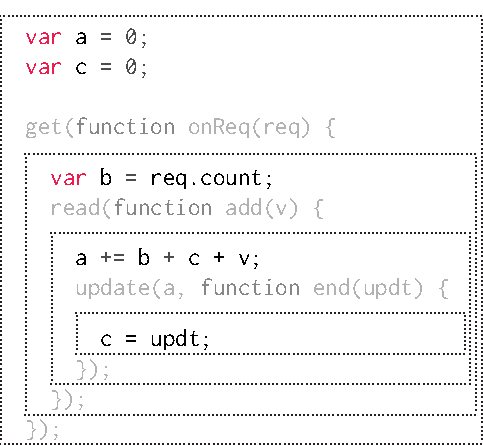
\includegraphics[width=\linewidth]{../resources/states.pdf}
  \caption{Variable management from Javascript to the high-level fluxionnal language}
  \label{fig:states}
\end{figure}

\paragraph{Scope}
If a variable is modified inside only one application part in the current \textit{post} chain, then the pipeliner adds it to the context of its fluxion.

In figure \ref{fig:states}, the variable \texttt{a} is updated in the function \texttt{add}.
The pipeliner step stores this variable in the context of the fluxion \texttt{add}.

\paragraph{Stream}
If a modified variable is read by downstream application parts, then the pipeliner makes the upstream fluxion add this variable to the message stream to be sent to the downstream fluxions.
It is impossible to send variables to upstream flux\-ions, without causing inconsistencies.
If the fluxion retro propagates the variable for an upstream fluxion to read, the upstream fluxion might use the old version while the new version is on its way.

In figure \ref{fig:states}, the variable \texttt{b} is set in the function \texttt{onReq}, and read in the function \texttt{add}.
The pipeliner step makes the fluxion \texttt{onReq} send the updated variable \texttt{b}, in addition to the variable \texttt{v}, in the message sent to the fluxion \texttt{add}.

Exceptionally, if a variable is defined inside a \textit{post} chain, like \texttt{b}, then this variable can be streamed inside this \textit{post} chain without restriction on the order of modification and read.
Indeed, the execution of the upstream fluxion for the current \textit{post} chain is assured to end before the execution of the downstream fluxion.
Therefore, no reading of the variable by the upstream fluxion happens after the modification by the downstream fluxion.

\paragraph{Share}
If a variable is needed for modification by several application parts, or is read by an upstream application part, then it needs to be synchronized between the fluxions.
To respect the semantics of the source application, we cannot tolerate inconsistencies.
Therefore, the pipeliner groups all the fluxions sharing this variable with the same tag.
And it adds this variable to the contexts of each fluxions.

In figure \ref{fig:states}, the variable \texttt{c} is set in the function \texttt{end}, and read in the function \texttt{add}.
As the fluxion \texttt{add} is upstream of \texttt{end}, the pipeliner step groups the fluxion \texttt{add} and \texttt{end} with the tag \texttt{grp\_c} to allow the two fluxions to share this variable.
\section{Overall Evaluation} \label{chapter6:evaluation}

The equivalence presented in chapter \ref{chapter4} is implemented in a the fluxional compiler, presented in section \ref{chapter5:flx}.
This implementation is evaluated against the criteria presented in chapter \ref{chapter3}, Productivity, Efficiency and Adoption.

\subsection{Trading Productivity for Efficiency}

% \subsubsection{Productivity}

The equivalence intends to disrupt as less as possible the way developer build web applications.
The goal is to avoid degrading the productivity, hence the adoption, of the proposed platform.
% The source language, Javascript, is left intact, except for the forbidden statements \texttt{with} and \texttt{eval}.
% These statements are already forbidden by some good practice guides \cite{Crockford2008}.
Therefore, the productivity is intended to be the same as the original event-driven platform.

However, in the current state, the compiler implementation is unable to operate the transformation without an external help.
The static analysis is unable to correctly detect the aliasing of the memory in Javascript.
It avoids developers to use Higher-Order Programming, hence impacts composition.
This limitation avoids to improve the current trade-off of productivity for efficiency, as illustrated in table \ref{tab:proposition-productivity}.
Indeed, to gain efficiency, developers need to commit efforts to indicate the stages of the pipeline, and assure their dependency.

% \TablePropositionProductivity{tab:proposition-productivity}

The manual transformation process yields a distributed application, similarly as the other efficient platforms.
And the chapter \ref{chapter3} showed that such applications achieve very good performance efficiency.
But the productivity limitation remains.
It avoids the current implementation to propose a satisfying compromise between productivity and efficiency.
So, the current implementation actually trades productivity for efficiency, similarly to many platform in the state of the art. % , as illustrated in table \ref{tab:proposition-efficiency}.
The perspectives to overcome this limitation are addressed later in section \ref{chapter5:evaluation:perspective}.
% \TablePropositionEfficiency{tab:proposition-efficiency}


% It doesn't make any sense to evaluate an application, as the transformation would not reflect the compilation process, but the manual transformation process.

% If the runtime memory analysis is solid enough to detect correctly the aliasing of the memory, then it will be able to help the development team transitioning from productivity to efficiency, which is the response of this thesis to the problematic.

\subsection{Adoption}

As observed in the chapter \ref{chapter3}, trading productivity for efficiency drastically reduces adoption.
Because the current implementation presents the same limitation than the efficient platforms, its adoption is not expected to be different. %, as illustrated in table \ref{tab:proposition-adoption}.

Yet, both productivity and efficiency are required for the platform to be adopted by new developers as well as large businesses.
Only at this condition, will it reinforce the loop between community and industry.
So the current implementation is not expected to be widely adopted, as presented in the table \ref{tab:proposition-summary}.

\TablePropositionSummary{tab:proposition-summary}
% \TablePropositionAdoption{tab:proposition-adoption}

% It was briefly tested during the development of the grumpy application, presented in chapter \ref{chapter4}, section \ref{chapter4:execution-models:examples}.

The limitation of static analysis avoids the equivalence to be fully implemented to address the problematic.
Hence, this evaluation holds only on the implementation, and not on the equivalence.


When saying that \textit{it is a mistake to attempt high concurrency without help from the compiler}, R. von Behren \textit{et al.} \cite{Behren2003} implies that the language alone cannot achieve high concurrency.
It is necessary to rely on additional tools, such as a compiler to reach the best compromise between productivity and efficiency.
The evaluation of this thesis concludes that static analysis is unable to reach this compromise for the current multi-paradigm languages using higher-order programming.
% Before dropping all higher-order languages for the sake of efficiency,
Yet, there exist alternatives to static analysis to reach this compromise.
The next paragraph presents some interesting perspectives of this work to further address this problematic.

% In the contribution of this thesis, the two main difficulties, identifying stages and detecting memory dependencies, are due to the dynamic nature of Javascript.
% A perspective to overcome these limitation is to implement the transformation, not as a compiler, but as a runtime.
% Indeed, at runtime, all the dynamic behavior are resolved, and the analysis can be much more precise, and less speculative.

% \subsection{Fluxionnal Runtime} 

% \section{Perspectives}

% Javascript is a highly dynamic languages.

\tableofcontents

\section{Fluxions} \label{chapter5:flx}

The previous section presented a compiler to identify and extract the underlying pipeline in a Javascript application.
However, the stages doesn't enforce the isolation required for parallel execution.
Moreover, the Dues that constitues the stages of this pipeline 

only parts of the pipeline are identified, 
This section present the second contribution of this thesis.
The equivalence between a memory shared among all the operations and independent memory for each operation in a pipeline.
It tackles the problems arising from the translation of the global memory synchronization into message passing.

This equivalence is implemented as a compiler, improving upon the previous one.
The compiler transforms a Javascript application into a network of independent parts communicating by message streams and executed in parallel.
We named these parts \textit{fluxions}, by contraction between a flux and a function.
% Fluxions are executed in an execution model that assure parallelism and communications.

% We present an early version of this tool as a proof of concept for this compilation approach.
% Section \ref{chapter5:flx:model} describes the execution model that executes fluxions in parallel, and assure their communications.

The identification of the rupture points between fluxions is addressed in section \ref{chapter5:flx:compiler}.
The isolation between the fluxions, after identification, is addressed in section \ref{chapter5:flx:isolation}.
% The compiler, and the equivalence are described in section \ref{chapter5:flx:compiler}.
Section \ref{chapter5:flx:evaluation} presents a real-case test of compilation, and expose the limits of this compiler.

# Explanation of the concept

## Turn-based programming.







(see presentation on Dues)
-> single-thread, no wait, no block and so on
Shared heap -> no mutex, no synchronization, so it is good scalability


Turn-based programming is an event-loop.
It is the execution of queued events one after the other.
An event is the association of a callback and a message.
The callback is a small Javascript Program, designed to process the message.
During its turn, the callback executes, and can queue events : that is register callback to be executed during a next turn.
TODO what I mean exactly by queue events ? -> the distinction between the asynchronous operation, and the resulting event.

## Pipeline

So a callback sends messages to other callbacks.
-> It is exactly like a pipeline.
However, all the callbacks share the same heap.
So it is not possible to distribute the different callbacks without synchronization of this heap, or splitting the heap for each callback.
TODO state VERY clearly this problem, it is at the core of my thesis.

So, how to split the heap so that each callback has its own exclusive heap ?

## Propagation of variables.

Javascript is lexically scoped, therefore we can identify the scope of variable statically.
(At the exception of eval and with : with is forbidden from strict mode, so that is not a bigdeal, howether, eval is sometimes used in smart ways, but most of the time it is monomorphic (I don't exactly know what that means, I heard from Floreat, it must be something related to PL community)).

### Scope identification

The compiler identifies the variables shared by multiple callbacks from their scope.
TODO explain this in depth.
Function scope, closures, and so on ...

### Scope leaking

Javascript uses a pass-by-sharing paradigm.
That means that sometimes the argument of a call are passed by value, sometimes by reference (atomic data type (number, string, bool) -> by value, complex data type (objects) -> by reference).
That means that the modification of a local variable can affect variable in seemingly unrelated scopes.
It seems that the points-to analysis is what is used to find stuffs like that (side-effects ?).

### Propagation of execution and variables

The execution progress downstream, following the message stream.
TODO state very clearly this proposition, it is the second core of my thesis (and I love the idea, it relates directly to reality, graivity, and the fabric of the universe <3).

Because the propagation of the modification is not instantaneous, going back upstream is like going backward in time : it is impossible.
Therefore, a variable cannot be read upstream a write.
And it cannot be write downstream either.

In other words, only one callback can write on a variable -> seems obvious from previous sections.


In promises, because the heap is not shared, things are less restrictive.
Multiple stages can read and write the same variable, because the propagation of modification is instantaneous, due to the shared heap.
\subsection{Fluxions Isolation} \label{chapter5:flx:isolation}

A rupture point eventually breaks the chain of scopes between the upstream and downstream fluxion.
The closure in the downstream fluxion cannot access the scope in the upstream fluxion as expected.
The pipeliner step replaces the need for this closure, allowing application parts to rely only on independent memory stores and message passing.
It determines the distribution using the scope representation, which represents the variables' dependencies between application parts.
Depending on this representation, the compiler can replace the broken closures in three different ways.
We present these three alternatives in figure \ref{fig:states}.

\begin{figure}[h!]
  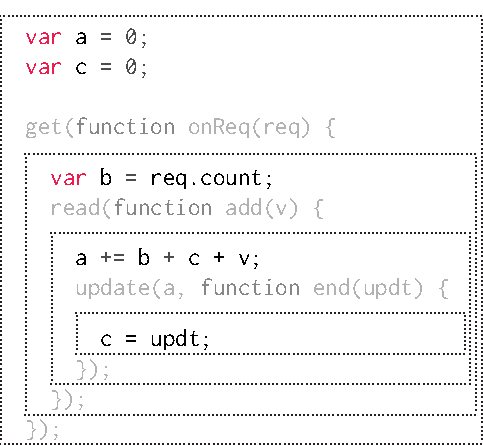
\includegraphics[width=\linewidth]{../resources/states.pdf}
  \caption{Variable management from Javascript to the high-level fluxionnal language}
  \label{fig:states}
\end{figure}

\paragraph{Scope}
If a variable is modified inside only one application part in the current \textit{post} chain, then the pipeliner adds it to the context of its fluxion.

In figure \ref{fig:states}, the variable \texttt{a} is updated in the function \texttt{add}.
The pipeliner step stores this variable in the context of the fluxion \texttt{add}.

\paragraph{Stream}
If a modified variable is read by downstream application parts, then the pipeliner makes the upstream fluxion add this variable to the message stream to be sent to the downstream fluxions.
It is impossible to send variables to upstream flux\-ions, without causing inconsistencies.
If the fluxion retro propagates the variable for an upstream fluxion to read, the upstream fluxion might use the old version while the new version is on its way.

In figure \ref{fig:states}, the variable \texttt{b} is set in the function \texttt{onReq}, and read in the function \texttt{add}.
The pipeliner step makes the fluxion \texttt{onReq} send the updated variable \texttt{b}, in addition to the variable \texttt{v}, in the message sent to the fluxion \texttt{add}.

Exceptionally, if a variable is defined inside a \textit{post} chain, like \texttt{b}, then this variable can be streamed inside this \textit{post} chain without restriction on the order of modification and read.
Indeed, the execution of the upstream fluxion for the current \textit{post} chain is assured to end before the execution of the downstream fluxion.
Therefore, no reading of the variable by the upstream fluxion happens after the modification by the downstream fluxion.

\paragraph{Share}
If a variable is needed for modification by several application parts, or is read by an upstream application part, then it needs to be synchronized between the fluxions.
To respect the semantics of the source application, we cannot tolerate inconsistencies.
Therefore, the pipeliner groups all the fluxions sharing this variable with the same tag.
And it adds this variable to the contexts of each fluxions.

In figure \ref{fig:states}, the variable \texttt{c} is set in the function \texttt{end}, and read in the function \texttt{add}.
As the fluxion \texttt{add} is upstream of \texttt{end}, the pipeliner step groups the fluxion \texttt{add} and \texttt{end} with the tag \texttt{grp\_c} to allow the two fluxions to share this variable.
\section{Overall Evaluation} \label{chapter6:evaluation}

The equivalence presented in chapter \ref{chapter4} is implemented in a the fluxional compiler, presented in section \ref{chapter5:flx}.
This implementation is evaluated against the criteria presented in chapter \ref{chapter3}, Productivity, Efficiency and Adoption.

\subsection{Trading Productivity for Efficiency}

% \subsubsection{Productivity}

The equivalence intends to disrupt as less as possible the way developer build web applications.
The goal is to avoid degrading the productivity, hence the adoption, of the proposed platform.
% The source language, Javascript, is left intact, except for the forbidden statements \texttt{with} and \texttt{eval}.
% These statements are already forbidden by some good practice guides \cite{Crockford2008}.
Therefore, the productivity is intended to be the same as the original event-driven platform.

However, in the current state, the compiler implementation is unable to operate the transformation without an external help.
The static analysis is unable to correctly detect the aliasing of the memory in Javascript.
It avoids developers to use Higher-Order Programming, hence impacts composition.
This limitation avoids to improve the current trade-off of productivity for efficiency, as illustrated in table \ref{tab:proposition-productivity}.
Indeed, to gain efficiency, developers need to commit efforts to indicate the stages of the pipeline, and assure their dependency.

% \TablePropositionProductivity{tab:proposition-productivity}

The manual transformation process yields a distributed application, similarly as the other efficient platforms.
And the chapter \ref{chapter3} showed that such applications achieve very good performance efficiency.
But the productivity limitation remains.
It avoids the current implementation to propose a satisfying compromise between productivity and efficiency.
So, the current implementation actually trades productivity for efficiency, similarly to many platform in the state of the art. % , as illustrated in table \ref{tab:proposition-efficiency}.
The perspectives to overcome this limitation are addressed later in section \ref{chapter5:evaluation:perspective}.
% \TablePropositionEfficiency{tab:proposition-efficiency}


% It doesn't make any sense to evaluate an application, as the transformation would not reflect the compilation process, but the manual transformation process.

% If the runtime memory analysis is solid enough to detect correctly the aliasing of the memory, then it will be able to help the development team transitioning from productivity to efficiency, which is the response of this thesis to the problematic.

\subsection{Adoption}

As observed in the chapter \ref{chapter3}, trading productivity for efficiency drastically reduces adoption.
Because the current implementation presents the same limitation than the efficient platforms, its adoption is not expected to be different. %, as illustrated in table \ref{tab:proposition-adoption}.

Yet, both productivity and efficiency are required for the platform to be adopted by new developers as well as large businesses.
Only at this condition, will it reinforce the loop between community and industry.
So the current implementation is not expected to be widely adopted, as presented in the table \ref{tab:proposition-summary}.

\TablePropositionSummary{tab:proposition-summary}
% \TablePropositionAdoption{tab:proposition-adoption}

% It was briefly tested during the development of the grumpy application, presented in chapter \ref{chapter4}, section \ref{chapter4:execution-models:examples}.

The limitation of static analysis avoids the equivalence to be fully implemented to address the problematic.
Hence, this evaluation holds only on the implementation, and not on the equivalence.


When saying that \textit{it is a mistake to attempt high concurrency without help from the compiler}, R. von Behren \textit{et al.} \cite{Behren2003} implies that the language alone cannot achieve high concurrency.
It is necessary to rely on additional tools, such as a compiler to reach the best compromise between productivity and efficiency.
The evaluation of this thesis concludes that static analysis is unable to reach this compromise for the current multi-paradigm languages using higher-order programming.
% Before dropping all higher-order languages for the sake of efficiency,
Yet, there exist alternatives to static analysis to reach this compromise.
The next paragraph presents some interesting perspectives of this work to further address this problematic.

% In the contribution of this thesis, the two main difficulties, identifying stages and detecting memory dependencies, are due to the dynamic nature of Javascript.
% A perspective to overcome these limitation is to implement the transformation, not as a compiler, but as a runtime.
% Indeed, at runtime, all the dynamic behavior are resolved, and the analysis can be much more precise, and less speculative.

% \subsection{Fluxionnal Runtime} 

% \section{Perspectives}

% Javascript is a highly dynamic languages.
\section{Fluxions} \label{chapter5:flx}

The previous section presented a compiler to identify and extract the underlying pipeline in a Javascript application.
However, the stages doesn't enforce the isolation required for parallel execution.
Moreover, the Dues that constitues the stages of this pipeline 

only parts of the pipeline are identified, 
This section present the second contribution of this thesis.
The equivalence between a memory shared among all the operations and independent memory for each operation in a pipeline.
It tackles the problems arising from the translation of the global memory synchronization into message passing.

This equivalence is implemented as a compiler, improving upon the previous one.
The compiler transforms a Javascript application into a network of independent parts communicating by message streams and executed in parallel.
We named these parts \textit{fluxions}, by contraction between a flux and a function.
% Fluxions are executed in an execution model that assure parallelism and communications.

% We present an early version of this tool as a proof of concept for this compilation approach.
% Section \ref{chapter5:flx:model} describes the execution model that executes fluxions in parallel, and assure their communications.

The identification of the rupture points between fluxions is addressed in section \ref{chapter5:flx:compiler}.
The isolation between the fluxions, after identification, is addressed in section \ref{chapter5:flx:isolation}.
% The compiler, and the equivalence are described in section \ref{chapter5:flx:compiler}.
Section \ref{chapter5:flx:evaluation} presents a real-case test of compilation, and expose the limits of this compiler.

# Explanation of the concept

## Turn-based programming.







(see presentation on Dues)
-> single-thread, no wait, no block and so on
Shared heap -> no mutex, no synchronization, so it is good scalability


Turn-based programming is an event-loop.
It is the execution of queued events one after the other.
An event is the association of a callback and a message.
The callback is a small Javascript Program, designed to process the message.
During its turn, the callback executes, and can queue events : that is register callback to be executed during a next turn.
TODO what I mean exactly by queue events ? -> the distinction between the asynchronous operation, and the resulting event.

## Pipeline

So a callback sends messages to other callbacks.
-> It is exactly like a pipeline.
However, all the callbacks share the same heap.
So it is not possible to distribute the different callbacks without synchronization of this heap, or splitting the heap for each callback.
TODO state VERY clearly this problem, it is at the core of my thesis.

So, how to split the heap so that each callback has its own exclusive heap ?

## Propagation of variables.

Javascript is lexically scoped, therefore we can identify the scope of variable statically.
(At the exception of eval and with : with is forbidden from strict mode, so that is not a bigdeal, howether, eval is sometimes used in smart ways, but most of the time it is monomorphic (I don't exactly know what that means, I heard from Floreat, it must be something related to PL community)).

### Scope identification

The compiler identifies the variables shared by multiple callbacks from their scope.
TODO explain this in depth.
Function scope, closures, and so on ...

### Scope leaking

Javascript uses a pass-by-sharing paradigm.
That means that sometimes the argument of a call are passed by value, sometimes by reference (atomic data type (number, string, bool) -> by value, complex data type (objects) -> by reference).
That means that the modification of a local variable can affect variable in seemingly unrelated scopes.
It seems that the points-to analysis is what is used to find stuffs like that (side-effects ?).

### Propagation of execution and variables

The execution progress downstream, following the message stream.
TODO state very clearly this proposition, it is the second core of my thesis (and I love the idea, it relates directly to reality, graivity, and the fabric of the universe <3).

Because the propagation of the modification is not instantaneous, going back upstream is like going backward in time : it is impossible.
Therefore, a variable cannot be read upstream a write.
And it cannot be write downstream either.

In other words, only one callback can write on a variable -> seems obvious from previous sections.


In promises, because the heap is not shared, things are less restrictive.
Multiple stages can read and write the same variable, because the propagation of modification is instantaneous, due to the shared heap.
\subsection{Fluxions Isolation} \label{chapter5:flx:isolation}

A rupture point eventually breaks the chain of scopes between the upstream and downstream fluxion.
The closure in the downstream fluxion cannot access the scope in the upstream fluxion as expected.
The pipeliner step replaces the need for this closure, allowing application parts to rely only on independent memory stores and message passing.
It determines the distribution using the scope representation, which represents the variables' dependencies between application parts.
Depending on this representation, the compiler can replace the broken closures in three different ways.
We present these three alternatives in figure \ref{fig:states}.

\begin{figure}[h!]
  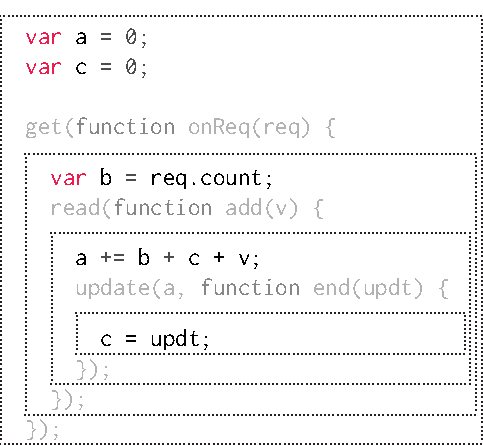
\includegraphics[width=\linewidth]{../resources/states.pdf}
  \caption{Variable management from Javascript to the high-level fluxionnal language}
  \label{fig:states}
\end{figure}

\paragraph{Scope}
If a variable is modified inside only one application part in the current \textit{post} chain, then the pipeliner adds it to the context of its fluxion.

In figure \ref{fig:states}, the variable \texttt{a} is updated in the function \texttt{add}.
The pipeliner step stores this variable in the context of the fluxion \texttt{add}.

\paragraph{Stream}
If a modified variable is read by downstream application parts, then the pipeliner makes the upstream fluxion add this variable to the message stream to be sent to the downstream fluxions.
It is impossible to send variables to upstream flux\-ions, without causing inconsistencies.
If the fluxion retro propagates the variable for an upstream fluxion to read, the upstream fluxion might use the old version while the new version is on its way.

In figure \ref{fig:states}, the variable \texttt{b} is set in the function \texttt{onReq}, and read in the function \texttt{add}.
The pipeliner step makes the fluxion \texttt{onReq} send the updated variable \texttt{b}, in addition to the variable \texttt{v}, in the message sent to the fluxion \texttt{add}.

Exceptionally, if a variable is defined inside a \textit{post} chain, like \texttt{b}, then this variable can be streamed inside this \textit{post} chain without restriction on the order of modification and read.
Indeed, the execution of the upstream fluxion for the current \textit{post} chain is assured to end before the execution of the downstream fluxion.
Therefore, no reading of the variable by the upstream fluxion happens after the modification by the downstream fluxion.

\paragraph{Share}
If a variable is needed for modification by several application parts, or is read by an upstream application part, then it needs to be synchronized between the fluxions.
To respect the semantics of the source application, we cannot tolerate inconsistencies.
Therefore, the pipeliner groups all the fluxions sharing this variable with the same tag.
And it adds this variable to the contexts of each fluxions.

In figure \ref{fig:states}, the variable \texttt{c} is set in the function \texttt{end}, and read in the function \texttt{add}.
As the fluxion \texttt{add} is upstream of \texttt{end}, the pipeliner step groups the fluxion \texttt{add} and \texttt{end} with the tag \texttt{grp\_c} to allow the two fluxions to share this variable.
\section{Overall Evaluation} \label{chapter6:evaluation}

The equivalence presented in chapter \ref{chapter4} is implemented in a the fluxional compiler, presented in section \ref{chapter5:flx}.
This implementation is evaluated against the criteria presented in chapter \ref{chapter3}, Productivity, Efficiency and Adoption.

\subsection{Trading Productivity for Efficiency}

% \subsubsection{Productivity}

The equivalence intends to disrupt as less as possible the way developer build web applications.
The goal is to avoid degrading the productivity, hence the adoption, of the proposed platform.
% The source language, Javascript, is left intact, except for the forbidden statements \texttt{with} and \texttt{eval}.
% These statements are already forbidden by some good practice guides \cite{Crockford2008}.
Therefore, the productivity is intended to be the same as the original event-driven platform.

However, in the current state, the compiler implementation is unable to operate the transformation without an external help.
The static analysis is unable to correctly detect the aliasing of the memory in Javascript.
It avoids developers to use Higher-Order Programming, hence impacts composition.
This limitation avoids to improve the current trade-off of productivity for efficiency, as illustrated in table \ref{tab:proposition-productivity}.
Indeed, to gain efficiency, developers need to commit efforts to indicate the stages of the pipeline, and assure their dependency.

% \TablePropositionProductivity{tab:proposition-productivity}

The manual transformation process yields a distributed application, similarly as the other efficient platforms.
And the chapter \ref{chapter3} showed that such applications achieve very good performance efficiency.
But the productivity limitation remains.
It avoids the current implementation to propose a satisfying compromise between productivity and efficiency.
So, the current implementation actually trades productivity for efficiency, similarly to many platform in the state of the art. % , as illustrated in table \ref{tab:proposition-efficiency}.
The perspectives to overcome this limitation are addressed later in section \ref{chapter5:evaluation:perspective}.
% \TablePropositionEfficiency{tab:proposition-efficiency}


% It doesn't make any sense to evaluate an application, as the transformation would not reflect the compilation process, but the manual transformation process.

% If the runtime memory analysis is solid enough to detect correctly the aliasing of the memory, then it will be able to help the development team transitioning from productivity to efficiency, which is the response of this thesis to the problematic.

\subsection{Adoption}

As observed in the chapter \ref{chapter3}, trading productivity for efficiency drastically reduces adoption.
Because the current implementation presents the same limitation than the efficient platforms, its adoption is not expected to be different. %, as illustrated in table \ref{tab:proposition-adoption}.

Yet, both productivity and efficiency are required for the platform to be adopted by new developers as well as large businesses.
Only at this condition, will it reinforce the loop between community and industry.
So the current implementation is not expected to be widely adopted, as presented in the table \ref{tab:proposition-summary}.

\TablePropositionSummary{tab:proposition-summary}
% \TablePropositionAdoption{tab:proposition-adoption}

% It was briefly tested during the development of the grumpy application, presented in chapter \ref{chapter4}, section \ref{chapter4:execution-models:examples}.

The limitation of static analysis avoids the equivalence to be fully implemented to address the problematic.
Hence, this evaluation holds only on the implementation, and not on the equivalence.


When saying that \textit{it is a mistake to attempt high concurrency without help from the compiler}, R. von Behren \textit{et al.} \cite{Behren2003} implies that the language alone cannot achieve high concurrency.
It is necessary to rely on additional tools, such as a compiler to reach the best compromise between productivity and efficiency.
The evaluation of this thesis concludes that static analysis is unable to reach this compromise for the current multi-paradigm languages using higher-order programming.
% Before dropping all higher-order languages for the sake of efficiency,
Yet, there exist alternatives to static analysis to reach this compromise.
The next paragraph presents some interesting perspectives of this work to further address this problematic.

% In the contribution of this thesis, the two main difficulties, identifying stages and detecting memory dependencies, are due to the dynamic nature of Javascript.
% A perspective to overcome these limitation is to implement the transformation, not as a compiler, but as a runtime.
% Indeed, at runtime, all the dynamic behavior are resolved, and the analysis can be much more precise, and less speculative.

% \subsection{Fluxionnal Runtime} 

% \section{Perspectives}

% Javascript is a highly dynamic languages.

% \section{Fluxions} \label{chapter5:flx}

The previous section presented a compiler to identify and extract the underlying pipeline in a Javascript application.
However, the stages doesn't enforce the isolation required for parallel execution.
Moreover, the Dues that constitues the stages of this pipeline 

only parts of the pipeline are identified, 
This section present the second contribution of this thesis.
The equivalence between a memory shared among all the operations and independent memory for each operation in a pipeline.
It tackles the problems arising from the translation of the global memory synchronization into message passing.

This equivalence is implemented as a compiler, improving upon the previous one.
The compiler transforms a Javascript application into a network of independent parts communicating by message streams and executed in parallel.
We named these parts \textit{fluxions}, by contraction between a flux and a function.
% Fluxions are executed in an execution model that assure parallelism and communications.

% We present an early version of this tool as a proof of concept for this compilation approach.
% Section \ref{chapter5:flx:model} describes the execution model that executes fluxions in parallel, and assure their communications.

The identification of the rupture points between fluxions is addressed in section \ref{chapter5:flx:compiler}.
The isolation between the fluxions, after identification, is addressed in section \ref{chapter5:flx:isolation}.
% The compiler, and the equivalence are described in section \ref{chapter5:flx:compiler}.
Section \ref{chapter5:flx:evaluation} presents a real-case test of compilation, and expose the limits of this compiler.

# Explanation of the concept

## Turn-based programming.







(see presentation on Dues)
-> single-thread, no wait, no block and so on
Shared heap -> no mutex, no synchronization, so it is good scalability


Turn-based programming is an event-loop.
It is the execution of queued events one after the other.
An event is the association of a callback and a message.
The callback is a small Javascript Program, designed to process the message.
During its turn, the callback executes, and can queue events : that is register callback to be executed during a next turn.
TODO what I mean exactly by queue events ? -> the distinction between the asynchronous operation, and the resulting event.

## Pipeline

So a callback sends messages to other callbacks.
-> It is exactly like a pipeline.
However, all the callbacks share the same heap.
So it is not possible to distribute the different callbacks without synchronization of this heap, or splitting the heap for each callback.
TODO state VERY clearly this problem, it is at the core of my thesis.

So, how to split the heap so that each callback has its own exclusive heap ?

## Propagation of variables.

Javascript is lexically scoped, therefore we can identify the scope of variable statically.
(At the exception of eval and with : with is forbidden from strict mode, so that is not a bigdeal, howether, eval is sometimes used in smart ways, but most of the time it is monomorphic (I don't exactly know what that means, I heard from Floreat, it must be something related to PL community)).

### Scope identification

The compiler identifies the variables shared by multiple callbacks from their scope.
TODO explain this in depth.
Function scope, closures, and so on ...

### Scope leaking

Javascript uses a pass-by-sharing paradigm.
That means that sometimes the argument of a call are passed by value, sometimes by reference (atomic data type (number, string, bool) -> by value, complex data type (objects) -> by reference).
That means that the modification of a local variable can affect variable in seemingly unrelated scopes.
It seems that the points-to analysis is what is used to find stuffs like that (side-effects ?).

### Propagation of execution and variables

The execution progress downstream, following the message stream.
TODO state very clearly this proposition, it is the second core of my thesis (and I love the idea, it relates directly to reality, graivity, and the fabric of the universe <3).

Because the propagation of the modification is not instantaneous, going back upstream is like going backward in time : it is impossible.
Therefore, a variable cannot be read upstream a write.
And it cannot be write downstream either.

In other words, only one callback can write on a variable -> seems obvious from previous sections.


In promises, because the heap is not shared, things are less restrictive.
Multiple stages can read and write the same variable, because the propagation of modification is instantaneous, due to the shared heap.
\subsection{Fluxions Isolation} \label{chapter5:flx:isolation}

A rupture point eventually breaks the chain of scopes between the upstream and downstream fluxion.
The closure in the downstream fluxion cannot access the scope in the upstream fluxion as expected.
The pipeliner step replaces the need for this closure, allowing application parts to rely only on independent memory stores and message passing.
It determines the distribution using the scope representation, which represents the variables' dependencies between application parts.
Depending on this representation, the compiler can replace the broken closures in three different ways.
We present these three alternatives in figure \ref{fig:states}.

\begin{figure}[h!]
  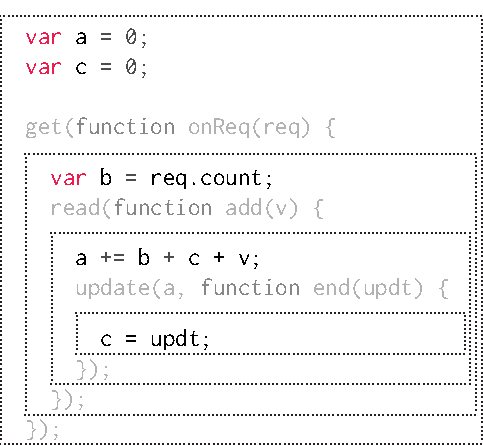
\includegraphics[width=\linewidth]{../resources/states.pdf}
  \caption{Variable management from Javascript to the high-level fluxionnal language}
  \label{fig:states}
\end{figure}

\paragraph{Scope}
If a variable is modified inside only one application part in the current \textit{post} chain, then the pipeliner adds it to the context of its fluxion.

In figure \ref{fig:states}, the variable \texttt{a} is updated in the function \texttt{add}.
The pipeliner step stores this variable in the context of the fluxion \texttt{add}.

\paragraph{Stream}
If a modified variable is read by downstream application parts, then the pipeliner makes the upstream fluxion add this variable to the message stream to be sent to the downstream fluxions.
It is impossible to send variables to upstream flux\-ions, without causing inconsistencies.
If the fluxion retro propagates the variable for an upstream fluxion to read, the upstream fluxion might use the old version while the new version is on its way.

In figure \ref{fig:states}, the variable \texttt{b} is set in the function \texttt{onReq}, and read in the function \texttt{add}.
The pipeliner step makes the fluxion \texttt{onReq} send the updated variable \texttt{b}, in addition to the variable \texttt{v}, in the message sent to the fluxion \texttt{add}.

Exceptionally, if a variable is defined inside a \textit{post} chain, like \texttt{b}, then this variable can be streamed inside this \textit{post} chain without restriction on the order of modification and read.
Indeed, the execution of the upstream fluxion for the current \textit{post} chain is assured to end before the execution of the downstream fluxion.
Therefore, no reading of the variable by the upstream fluxion happens after the modification by the downstream fluxion.

\paragraph{Share}
If a variable is needed for modification by several application parts, or is read by an upstream application part, then it needs to be synchronized between the fluxions.
To respect the semantics of the source application, we cannot tolerate inconsistencies.
Therefore, the pipeliner groups all the fluxions sharing this variable with the same tag.
And it adds this variable to the contexts of each fluxions.

In figure \ref{fig:states}, the variable \texttt{c} is set in the function \texttt{end}, and read in the function \texttt{add}.
As the fluxion \texttt{add} is upstream of \texttt{end}, the pipeliner step groups the fluxion \texttt{add} and \texttt{end} with the tag \texttt{grp\_c} to allow the two fluxions to share this variable.
\section{Overall Evaluation} \label{chapter6:evaluation}

The equivalence presented in chapter \ref{chapter4} is implemented in a the fluxional compiler, presented in section \ref{chapter5:flx}.
This implementation is evaluated against the criteria presented in chapter \ref{chapter3}, Productivity, Efficiency and Adoption.

\subsection{Trading Productivity for Efficiency}

% \subsubsection{Productivity}

The equivalence intends to disrupt as less as possible the way developer build web applications.
The goal is to avoid degrading the productivity, hence the adoption, of the proposed platform.
% The source language, Javascript, is left intact, except for the forbidden statements \texttt{with} and \texttt{eval}.
% These statements are already forbidden by some good practice guides \cite{Crockford2008}.
Therefore, the productivity is intended to be the same as the original event-driven platform.

However, in the current state, the compiler implementation is unable to operate the transformation without an external help.
The static analysis is unable to correctly detect the aliasing of the memory in Javascript.
It avoids developers to use Higher-Order Programming, hence impacts composition.
This limitation avoids to improve the current trade-off of productivity for efficiency, as illustrated in table \ref{tab:proposition-productivity}.
Indeed, to gain efficiency, developers need to commit efforts to indicate the stages of the pipeline, and assure their dependency.

% \TablePropositionProductivity{tab:proposition-productivity}

The manual transformation process yields a distributed application, similarly as the other efficient platforms.
And the chapter \ref{chapter3} showed that such applications achieve very good performance efficiency.
But the productivity limitation remains.
It avoids the current implementation to propose a satisfying compromise between productivity and efficiency.
So, the current implementation actually trades productivity for efficiency, similarly to many platform in the state of the art. % , as illustrated in table \ref{tab:proposition-efficiency}.
The perspectives to overcome this limitation are addressed later in section \ref{chapter5:evaluation:perspective}.
% \TablePropositionEfficiency{tab:proposition-efficiency}


% It doesn't make any sense to evaluate an application, as the transformation would not reflect the compilation process, but the manual transformation process.

% If the runtime memory analysis is solid enough to detect correctly the aliasing of the memory, then it will be able to help the development team transitioning from productivity to efficiency, which is the response of this thesis to the problematic.

\subsection{Adoption}

As observed in the chapter \ref{chapter3}, trading productivity for efficiency drastically reduces adoption.
Because the current implementation presents the same limitation than the efficient platforms, its adoption is not expected to be different. %, as illustrated in table \ref{tab:proposition-adoption}.

Yet, both productivity and efficiency are required for the platform to be adopted by new developers as well as large businesses.
Only at this condition, will it reinforce the loop between community and industry.
So the current implementation is not expected to be widely adopted, as presented in the table \ref{tab:proposition-summary}.

\TablePropositionSummary{tab:proposition-summary}
% \TablePropositionAdoption{tab:proposition-adoption}

% It was briefly tested during the development of the grumpy application, presented in chapter \ref{chapter4}, section \ref{chapter4:execution-models:examples}.

The limitation of static analysis avoids the equivalence to be fully implemented to address the problematic.
Hence, this evaluation holds only on the implementation, and not on the equivalence.


When saying that \textit{it is a mistake to attempt high concurrency without help from the compiler}, R. von Behren \textit{et al.} \cite{Behren2003} implies that the language alone cannot achieve high concurrency.
It is necessary to rely on additional tools, such as a compiler to reach the best compromise between productivity and efficiency.
The evaluation of this thesis concludes that static analysis is unable to reach this compromise for the current multi-paradigm languages using higher-order programming.
% Before dropping all higher-order languages for the sake of efficiency,
Yet, there exist alternatives to static analysis to reach this compromise.
The next paragraph presents some interesting perspectives of this work to further address this problematic.

% In the contribution of this thesis, the two main difficulties, identifying stages and detecting memory dependencies, are due to the dynamic nature of Javascript.
% A perspective to overcome these limitation is to implement the transformation, not as a compiler, but as a runtime.
% Indeed, at runtime, all the dynamic behavior are resolved, and the analysis can be much more precise, and less speculative.

% \subsection{Fluxionnal Runtime} 

% \section{Perspectives}

% Javascript is a highly dynamic languages.

%\chapter{A framework for parallel web applications}
 % \section{Fluxions}

\chapter{\comment{State of the art}}

  \section{Framworks for web application distribution}
    \subsection{Micro-batch processing}
    \subsection{Stream Processing}
  
  \section{Flow programming}
      \subsection{Functional reactive programming}
      \subsection{Flow-Based programming}
  \section{Parallelizing compilers}
    \comment{OpenMP and so on}
    %\subsubsection{\comment{TODO}}

  \section{\comment{Synthesis}}
    \comment{There is no compiler focusing on event-loop based applications}

\chapter{Fluxion}

  \section{Fluxionnal execution model}
    \subsection{Fluxion encapsulation}
      \subsubsection{Execution}
      \subsubsection{Name}
      \subsubsection{Memory}
    \subsection{Messaging system}

  \section{Fluxionnal Compiler}
    \subsection{Identification}
      \subsubsection{Continuation and listeners}
      \subsubsection{Dues}
    \subsection{Isolation}
      \subsubsection{Scope identification}
        \comment{Scope leaking}
      \subsubsection{Execution and variable propagation}
    \subsection{distribution}

\chapter{Evaluation}
  \section{Due compiler}
  \section{Fluxionnal compiler}
  \section{Fluxionnal execution model}

\section{Fluxions} \label{chapter5:flx}

The previous section presented a compiler to identify and extract the underlying pipeline in a Javascript application.
However, the stages doesn't enforce the isolation required for parallel execution.
Moreover, the Dues that constitues the stages of this pipeline 

only parts of the pipeline are identified, 
This section present the second contribution of this thesis.
The equivalence between a memory shared among all the operations and independent memory for each operation in a pipeline.
It tackles the problems arising from the translation of the global memory synchronization into message passing.

This equivalence is implemented as a compiler, improving upon the previous one.
The compiler transforms a Javascript application into a network of independent parts communicating by message streams and executed in parallel.
We named these parts \textit{fluxions}, by contraction between a flux and a function.
% Fluxions are executed in an execution model that assure parallelism and communications.

% We present an early version of this tool as a proof of concept for this compilation approach.
% Section \ref{chapter5:flx:model} describes the execution model that executes fluxions in parallel, and assure their communications.

The identification of the rupture points between fluxions is addressed in section \ref{chapter5:flx:compiler}.
The isolation between the fluxions, after identification, is addressed in section \ref{chapter5:flx:isolation}.
% The compiler, and the equivalence are described in section \ref{chapter5:flx:compiler}.
Section \ref{chapter5:flx:evaluation} presents a real-case test of compilation, and expose the limits of this compiler.

# Explanation of the concept

## Turn-based programming.







(see presentation on Dues)
-> single-thread, no wait, no block and so on
Shared heap -> no mutex, no synchronization, so it is good scalability


Turn-based programming is an event-loop.
It is the execution of queued events one after the other.
An event is the association of a callback and a message.
The callback is a small Javascript Program, designed to process the message.
During its turn, the callback executes, and can queue events : that is register callback to be executed during a next turn.
TODO what I mean exactly by queue events ? -> the distinction between the asynchronous operation, and the resulting event.

## Pipeline

So a callback sends messages to other callbacks.
-> It is exactly like a pipeline.
However, all the callbacks share the same heap.
So it is not possible to distribute the different callbacks without synchronization of this heap, or splitting the heap for each callback.
TODO state VERY clearly this problem, it is at the core of my thesis.

So, how to split the heap so that each callback has its own exclusive heap ?

## Propagation of variables.

Javascript is lexically scoped, therefore we can identify the scope of variable statically.
(At the exception of eval and with : with is forbidden from strict mode, so that is not a bigdeal, howether, eval is sometimes used in smart ways, but most of the time it is monomorphic (I don't exactly know what that means, I heard from Floreat, it must be something related to PL community)).

### Scope identification

The compiler identifies the variables shared by multiple callbacks from their scope.
TODO explain this in depth.
Function scope, closures, and so on ...

### Scope leaking

Javascript uses a pass-by-sharing paradigm.
That means that sometimes the argument of a call are passed by value, sometimes by reference (atomic data type (number, string, bool) -> by value, complex data type (objects) -> by reference).
That means that the modification of a local variable can affect variable in seemingly unrelated scopes.
It seems that the points-to analysis is what is used to find stuffs like that (side-effects ?).

### Propagation of execution and variables

The execution progress downstream, following the message stream.
TODO state very clearly this proposition, it is the second core of my thesis (and I love the idea, it relates directly to reality, graivity, and the fabric of the universe <3).

Because the propagation of the modification is not instantaneous, going back upstream is like going backward in time : it is impossible.
Therefore, a variable cannot be read upstream a write.
And it cannot be write downstream either.

In other words, only one callback can write on a variable -> seems obvious from previous sections.


In promises, because the heap is not shared, things are less restrictive.
Multiple stages can read and write the same variable, because the propagation of modification is instantaneous, due to the shared heap.
\subsection{Fluxions Isolation} \label{chapter5:flx:isolation}

A rupture point eventually breaks the chain of scopes between the upstream and downstream fluxion.
The closure in the downstream fluxion cannot access the scope in the upstream fluxion as expected.
The pipeliner step replaces the need for this closure, allowing application parts to rely only on independent memory stores and message passing.
It determines the distribution using the scope representation, which represents the variables' dependencies between application parts.
Depending on this representation, the compiler can replace the broken closures in three different ways.
We present these three alternatives in figure \ref{fig:states}.

\begin{figure}[h!]
  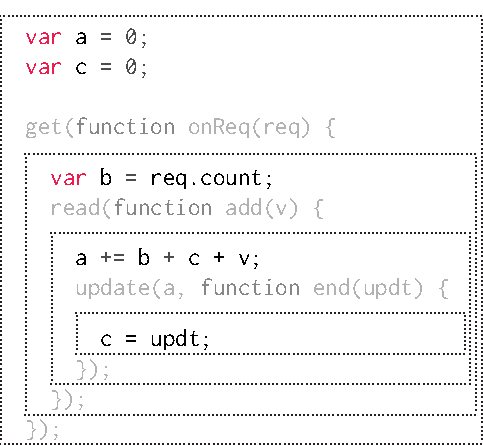
\includegraphics[width=\linewidth]{../resources/states.pdf}
  \caption{Variable management from Javascript to the high-level fluxionnal language}
  \label{fig:states}
\end{figure}

\paragraph{Scope}
If a variable is modified inside only one application part in the current \textit{post} chain, then the pipeliner adds it to the context of its fluxion.

In figure \ref{fig:states}, the variable \texttt{a} is updated in the function \texttt{add}.
The pipeliner step stores this variable in the context of the fluxion \texttt{add}.

\paragraph{Stream}
If a modified variable is read by downstream application parts, then the pipeliner makes the upstream fluxion add this variable to the message stream to be sent to the downstream fluxions.
It is impossible to send variables to upstream flux\-ions, without causing inconsistencies.
If the fluxion retro propagates the variable for an upstream fluxion to read, the upstream fluxion might use the old version while the new version is on its way.

In figure \ref{fig:states}, the variable \texttt{b} is set in the function \texttt{onReq}, and read in the function \texttt{add}.
The pipeliner step makes the fluxion \texttt{onReq} send the updated variable \texttt{b}, in addition to the variable \texttt{v}, in the message sent to the fluxion \texttt{add}.

Exceptionally, if a variable is defined inside a \textit{post} chain, like \texttt{b}, then this variable can be streamed inside this \textit{post} chain without restriction on the order of modification and read.
Indeed, the execution of the upstream fluxion for the current \textit{post} chain is assured to end before the execution of the downstream fluxion.
Therefore, no reading of the variable by the upstream fluxion happens after the modification by the downstream fluxion.

\paragraph{Share}
If a variable is needed for modification by several application parts, or is read by an upstream application part, then it needs to be synchronized between the fluxions.
To respect the semantics of the source application, we cannot tolerate inconsistencies.
Therefore, the pipeliner groups all the fluxions sharing this variable with the same tag.
And it adds this variable to the contexts of each fluxions.

In figure \ref{fig:states}, the variable \texttt{c} is set in the function \texttt{end}, and read in the function \texttt{add}.
As the fluxion \texttt{add} is upstream of \texttt{end}, the pipeliner step groups the fluxion \texttt{add} and \texttt{end} with the tag \texttt{grp\_c} to allow the two fluxions to share this variable.
\section{Overall Evaluation} \label{chapter6:evaluation}

The equivalence presented in chapter \ref{chapter4} is implemented in a the fluxional compiler, presented in section \ref{chapter5:flx}.
This implementation is evaluated against the criteria presented in chapter \ref{chapter3}, Productivity, Efficiency and Adoption.

\subsection{Trading Productivity for Efficiency}

% \subsubsection{Productivity}

The equivalence intends to disrupt as less as possible the way developer build web applications.
The goal is to avoid degrading the productivity, hence the adoption, of the proposed platform.
% The source language, Javascript, is left intact, except for the forbidden statements \texttt{with} and \texttt{eval}.
% These statements are already forbidden by some good practice guides \cite{Crockford2008}.
Therefore, the productivity is intended to be the same as the original event-driven platform.

However, in the current state, the compiler implementation is unable to operate the transformation without an external help.
The static analysis is unable to correctly detect the aliasing of the memory in Javascript.
It avoids developers to use Higher-Order Programming, hence impacts composition.
This limitation avoids to improve the current trade-off of productivity for efficiency, as illustrated in table \ref{tab:proposition-productivity}.
Indeed, to gain efficiency, developers need to commit efforts to indicate the stages of the pipeline, and assure their dependency.

% \TablePropositionProductivity{tab:proposition-productivity}

The manual transformation process yields a distributed application, similarly as the other efficient platforms.
And the chapter \ref{chapter3} showed that such applications achieve very good performance efficiency.
But the productivity limitation remains.
It avoids the current implementation to propose a satisfying compromise between productivity and efficiency.
So, the current implementation actually trades productivity for efficiency, similarly to many platform in the state of the art. % , as illustrated in table \ref{tab:proposition-efficiency}.
The perspectives to overcome this limitation are addressed later in section \ref{chapter5:evaluation:perspective}.
% \TablePropositionEfficiency{tab:proposition-efficiency}


% It doesn't make any sense to evaluate an application, as the transformation would not reflect the compilation process, but the manual transformation process.

% If the runtime memory analysis is solid enough to detect correctly the aliasing of the memory, then it will be able to help the development team transitioning from productivity to efficiency, which is the response of this thesis to the problematic.

\subsection{Adoption}

As observed in the chapter \ref{chapter3}, trading productivity for efficiency drastically reduces adoption.
Because the current implementation presents the same limitation than the efficient platforms, its adoption is not expected to be different. %, as illustrated in table \ref{tab:proposition-adoption}.

Yet, both productivity and efficiency are required for the platform to be adopted by new developers as well as large businesses.
Only at this condition, will it reinforce the loop between community and industry.
So the current implementation is not expected to be widely adopted, as presented in the table \ref{tab:proposition-summary}.

\TablePropositionSummary{tab:proposition-summary}
% \TablePropositionAdoption{tab:proposition-adoption}

% It was briefly tested during the development of the grumpy application, presented in chapter \ref{chapter4}, section \ref{chapter4:execution-models:examples}.

The limitation of static analysis avoids the equivalence to be fully implemented to address the problematic.
Hence, this evaluation holds only on the implementation, and not on the equivalence.


When saying that \textit{it is a mistake to attempt high concurrency without help from the compiler}, R. von Behren \textit{et al.} \cite{Behren2003} implies that the language alone cannot achieve high concurrency.
It is necessary to rely on additional tools, such as a compiler to reach the best compromise between productivity and efficiency.
The evaluation of this thesis concludes that static analysis is unable to reach this compromise for the current multi-paradigm languages using higher-order programming.
% Before dropping all higher-order languages for the sake of efficiency,
Yet, there exist alternatives to static analysis to reach this compromise.
The next paragraph presents some interesting perspectives of this work to further address this problematic.

% In the contribution of this thesis, the two main difficulties, identifying stages and detecting memory dependencies, are due to the dynamic nature of Javascript.
% A perspective to overcome these limitation is to implement the transformation, not as a compiler, but as a runtime.
% Indeed, at runtime, all the dynamic behavior are resolved, and the analysis can be much more precise, and less speculative.

% \subsection{Fluxionnal Runtime} 

% \section{Perspectives}

% Javascript is a highly dynamic languages.
\section{Fluxions} \label{chapter5:flx}

The previous section presented a compiler to identify and extract the underlying pipeline in a Javascript application.
However, the stages doesn't enforce the isolation required for parallel execution.
Moreover, the Dues that constitues the stages of this pipeline 

only parts of the pipeline are identified, 
This section present the second contribution of this thesis.
The equivalence between a memory shared among all the operations and independent memory for each operation in a pipeline.
It tackles the problems arising from the translation of the global memory synchronization into message passing.

This equivalence is implemented as a compiler, improving upon the previous one.
The compiler transforms a Javascript application into a network of independent parts communicating by message streams and executed in parallel.
We named these parts \textit{fluxions}, by contraction between a flux and a function.
% Fluxions are executed in an execution model that assure parallelism and communications.

% We present an early version of this tool as a proof of concept for this compilation approach.
% Section \ref{chapter5:flx:model} describes the execution model that executes fluxions in parallel, and assure their communications.

The identification of the rupture points between fluxions is addressed in section \ref{chapter5:flx:compiler}.
The isolation between the fluxions, after identification, is addressed in section \ref{chapter5:flx:isolation}.
% The compiler, and the equivalence are described in section \ref{chapter5:flx:compiler}.
Section \ref{chapter5:flx:evaluation} presents a real-case test of compilation, and expose the limits of this compiler.

# Explanation of the concept

## Turn-based programming.







(see presentation on Dues)
-> single-thread, no wait, no block and so on
Shared heap -> no mutex, no synchronization, so it is good scalability


Turn-based programming is an event-loop.
It is the execution of queued events one after the other.
An event is the association of a callback and a message.
The callback is a small Javascript Program, designed to process the message.
During its turn, the callback executes, and can queue events : that is register callback to be executed during a next turn.
TODO what I mean exactly by queue events ? -> the distinction between the asynchronous operation, and the resulting event.

## Pipeline

So a callback sends messages to other callbacks.
-> It is exactly like a pipeline.
However, all the callbacks share the same heap.
So it is not possible to distribute the different callbacks without synchronization of this heap, or splitting the heap for each callback.
TODO state VERY clearly this problem, it is at the core of my thesis.

So, how to split the heap so that each callback has its own exclusive heap ?

## Propagation of variables.

Javascript is lexically scoped, therefore we can identify the scope of variable statically.
(At the exception of eval and with : with is forbidden from strict mode, so that is not a bigdeal, howether, eval is sometimes used in smart ways, but most of the time it is monomorphic (I don't exactly know what that means, I heard from Floreat, it must be something related to PL community)).

### Scope identification

The compiler identifies the variables shared by multiple callbacks from their scope.
TODO explain this in depth.
Function scope, closures, and so on ...

### Scope leaking

Javascript uses a pass-by-sharing paradigm.
That means that sometimes the argument of a call are passed by value, sometimes by reference (atomic data type (number, string, bool) -> by value, complex data type (objects) -> by reference).
That means that the modification of a local variable can affect variable in seemingly unrelated scopes.
It seems that the points-to analysis is what is used to find stuffs like that (side-effects ?).

### Propagation of execution and variables

The execution progress downstream, following the message stream.
TODO state very clearly this proposition, it is the second core of my thesis (and I love the idea, it relates directly to reality, graivity, and the fabric of the universe <3).

Because the propagation of the modification is not instantaneous, going back upstream is like going backward in time : it is impossible.
Therefore, a variable cannot be read upstream a write.
And it cannot be write downstream either.

In other words, only one callback can write on a variable -> seems obvious from previous sections.


In promises, because the heap is not shared, things are less restrictive.
Multiple stages can read and write the same variable, because the propagation of modification is instantaneous, due to the shared heap.
\subsection{Fluxions Isolation} \label{chapter5:flx:isolation}

A rupture point eventually breaks the chain of scopes between the upstream and downstream fluxion.
The closure in the downstream fluxion cannot access the scope in the upstream fluxion as expected.
The pipeliner step replaces the need for this closure, allowing application parts to rely only on independent memory stores and message passing.
It determines the distribution using the scope representation, which represents the variables' dependencies between application parts.
Depending on this representation, the compiler can replace the broken closures in three different ways.
We present these three alternatives in figure \ref{fig:states}.

\begin{figure}[h!]
  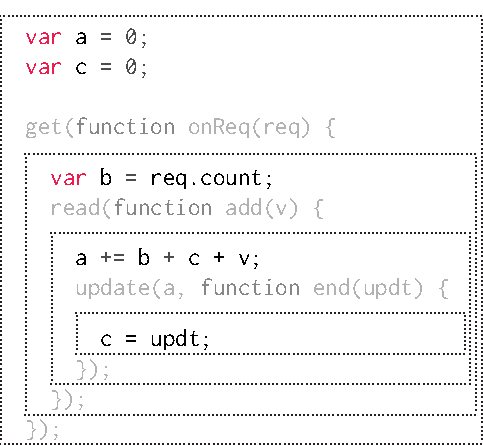
\includegraphics[width=\linewidth]{../resources/states.pdf}
  \caption{Variable management from Javascript to the high-level fluxionnal language}
  \label{fig:states}
\end{figure}

\paragraph{Scope}
If a variable is modified inside only one application part in the current \textit{post} chain, then the pipeliner adds it to the context of its fluxion.

In figure \ref{fig:states}, the variable \texttt{a} is updated in the function \texttt{add}.
The pipeliner step stores this variable in the context of the fluxion \texttt{add}.

\paragraph{Stream}
If a modified variable is read by downstream application parts, then the pipeliner makes the upstream fluxion add this variable to the message stream to be sent to the downstream fluxions.
It is impossible to send variables to upstream flux\-ions, without causing inconsistencies.
If the fluxion retro propagates the variable for an upstream fluxion to read, the upstream fluxion might use the old version while the new version is on its way.

In figure \ref{fig:states}, the variable \texttt{b} is set in the function \texttt{onReq}, and read in the function \texttt{add}.
The pipeliner step makes the fluxion \texttt{onReq} send the updated variable \texttt{b}, in addition to the variable \texttt{v}, in the message sent to the fluxion \texttt{add}.

Exceptionally, if a variable is defined inside a \textit{post} chain, like \texttt{b}, then this variable can be streamed inside this \textit{post} chain without restriction on the order of modification and read.
Indeed, the execution of the upstream fluxion for the current \textit{post} chain is assured to end before the execution of the downstream fluxion.
Therefore, no reading of the variable by the upstream fluxion happens after the modification by the downstream fluxion.

\paragraph{Share}
If a variable is needed for modification by several application parts, or is read by an upstream application part, then it needs to be synchronized between the fluxions.
To respect the semantics of the source application, we cannot tolerate inconsistencies.
Therefore, the pipeliner groups all the fluxions sharing this variable with the same tag.
And it adds this variable to the contexts of each fluxions.

In figure \ref{fig:states}, the variable \texttt{c} is set in the function \texttt{end}, and read in the function \texttt{add}.
As the fluxion \texttt{add} is upstream of \texttt{end}, the pipeliner step groups the fluxion \texttt{add} and \texttt{end} with the tag \texttt{grp\_c} to allow the two fluxions to share this variable.
\section{Overall Evaluation} \label{chapter6:evaluation}

The equivalence presented in chapter \ref{chapter4} is implemented in a the fluxional compiler, presented in section \ref{chapter5:flx}.
This implementation is evaluated against the criteria presented in chapter \ref{chapter3}, Productivity, Efficiency and Adoption.

\subsection{Trading Productivity for Efficiency}

% \subsubsection{Productivity}

The equivalence intends to disrupt as less as possible the way developer build web applications.
The goal is to avoid degrading the productivity, hence the adoption, of the proposed platform.
% The source language, Javascript, is left intact, except for the forbidden statements \texttt{with} and \texttt{eval}.
% These statements are already forbidden by some good practice guides \cite{Crockford2008}.
Therefore, the productivity is intended to be the same as the original event-driven platform.

However, in the current state, the compiler implementation is unable to operate the transformation without an external help.
The static analysis is unable to correctly detect the aliasing of the memory in Javascript.
It avoids developers to use Higher-Order Programming, hence impacts composition.
This limitation avoids to improve the current trade-off of productivity for efficiency, as illustrated in table \ref{tab:proposition-productivity}.
Indeed, to gain efficiency, developers need to commit efforts to indicate the stages of the pipeline, and assure their dependency.

% \TablePropositionProductivity{tab:proposition-productivity}

The manual transformation process yields a distributed application, similarly as the other efficient platforms.
And the chapter \ref{chapter3} showed that such applications achieve very good performance efficiency.
But the productivity limitation remains.
It avoids the current implementation to propose a satisfying compromise between productivity and efficiency.
So, the current implementation actually trades productivity for efficiency, similarly to many platform in the state of the art. % , as illustrated in table \ref{tab:proposition-efficiency}.
The perspectives to overcome this limitation are addressed later in section \ref{chapter5:evaluation:perspective}.
% \TablePropositionEfficiency{tab:proposition-efficiency}


% It doesn't make any sense to evaluate an application, as the transformation would not reflect the compilation process, but the manual transformation process.

% If the runtime memory analysis is solid enough to detect correctly the aliasing of the memory, then it will be able to help the development team transitioning from productivity to efficiency, which is the response of this thesis to the problematic.

\subsection{Adoption}

As observed in the chapter \ref{chapter3}, trading productivity for efficiency drastically reduces adoption.
Because the current implementation presents the same limitation than the efficient platforms, its adoption is not expected to be different. %, as illustrated in table \ref{tab:proposition-adoption}.

Yet, both productivity and efficiency are required for the platform to be adopted by new developers as well as large businesses.
Only at this condition, will it reinforce the loop between community and industry.
So the current implementation is not expected to be widely adopted, as presented in the table \ref{tab:proposition-summary}.

\TablePropositionSummary{tab:proposition-summary}
% \TablePropositionAdoption{tab:proposition-adoption}

% It was briefly tested during the development of the grumpy application, presented in chapter \ref{chapter4}, section \ref{chapter4:execution-models:examples}.

The limitation of static analysis avoids the equivalence to be fully implemented to address the problematic.
Hence, this evaluation holds only on the implementation, and not on the equivalence.


When saying that \textit{it is a mistake to attempt high concurrency without help from the compiler}, R. von Behren \textit{et al.} \cite{Behren2003} implies that the language alone cannot achieve high concurrency.
It is necessary to rely on additional tools, such as a compiler to reach the best compromise between productivity and efficiency.
The evaluation of this thesis concludes that static analysis is unable to reach this compromise for the current multi-paradigm languages using higher-order programming.
% Before dropping all higher-order languages for the sake of efficiency,
Yet, there exist alternatives to static analysis to reach this compromise.
The next paragraph presents some interesting perspectives of this work to further address this problematic.

% In the contribution of this thesis, the two main difficulties, identifying stages and detecting memory dependencies, are due to the dynamic nature of Javascript.
% A perspective to overcome these limitation is to implement the transformation, not as a compiler, but as a runtime.
% Indeed, at runtime, all the dynamic behavior are resolved, and the analysis can be much more precise, and less speculative.

% \subsection{Fluxionnal Runtime} 

% \section{Perspectives}

% Javascript is a highly dynamic languages.

\printbibliography[]

\end{document}